% Options for packages loaded elsewhere
\PassOptionsToPackage{unicode}{hyperref}
\PassOptionsToPackage{hyphens}{url}
%
\documentclass[
]{article}
\usepackage{amsmath,amssymb}
\usepackage{lmodern}
\usepackage{iftex}
\ifPDFTeX
  \usepackage[T1]{fontenc}
  \usepackage[utf8]{inputenc}
  \usepackage{textcomp} % provide euro and other symbols
\else % if luatex or xetex
  \usepackage{unicode-math}
  \defaultfontfeatures{Scale=MatchLowercase}
  \defaultfontfeatures[\rmfamily]{Ligatures=TeX,Scale=1}
\fi
% Use upquote if available, for straight quotes in verbatim environments
\IfFileExists{upquote.sty}{\usepackage{upquote}}{}
\IfFileExists{microtype.sty}{% use microtype if available
  \usepackage[]{microtype}
  \UseMicrotypeSet[protrusion]{basicmath} % disable protrusion for tt fonts
}{}
\makeatletter
\@ifundefined{KOMAClassName}{% if non-KOMA class
  \IfFileExists{parskip.sty}{%
    \usepackage{parskip}
  }{% else
    \setlength{\parindent}{0pt}
    \setlength{\parskip}{6pt plus 2pt minus 1pt}}
}{% if KOMA class
  \KOMAoptions{parskip=half}}
\makeatother
\usepackage{xcolor}
\usepackage[margin=1in]{geometry}
\usepackage{color}
\usepackage{fancyvrb}
\newcommand{\VerbBar}{|}
\newcommand{\VERB}{\Verb[commandchars=\\\{\}]}
\DefineVerbatimEnvironment{Highlighting}{Verbatim}{commandchars=\\\{\}}
% Add ',fontsize=\small' for more characters per line
\usepackage{framed}
\definecolor{shadecolor}{RGB}{248,248,248}
\newenvironment{Shaded}{\begin{snugshade}}{\end{snugshade}}
\newcommand{\AlertTok}[1]{\textcolor[rgb]{0.94,0.16,0.16}{#1}}
\newcommand{\AnnotationTok}[1]{\textcolor[rgb]{0.56,0.35,0.01}{\textbf{\textit{#1}}}}
\newcommand{\AttributeTok}[1]{\textcolor[rgb]{0.77,0.63,0.00}{#1}}
\newcommand{\BaseNTok}[1]{\textcolor[rgb]{0.00,0.00,0.81}{#1}}
\newcommand{\BuiltInTok}[1]{#1}
\newcommand{\CharTok}[1]{\textcolor[rgb]{0.31,0.60,0.02}{#1}}
\newcommand{\CommentTok}[1]{\textcolor[rgb]{0.56,0.35,0.01}{\textit{#1}}}
\newcommand{\CommentVarTok}[1]{\textcolor[rgb]{0.56,0.35,0.01}{\textbf{\textit{#1}}}}
\newcommand{\ConstantTok}[1]{\textcolor[rgb]{0.00,0.00,0.00}{#1}}
\newcommand{\ControlFlowTok}[1]{\textcolor[rgb]{0.13,0.29,0.53}{\textbf{#1}}}
\newcommand{\DataTypeTok}[1]{\textcolor[rgb]{0.13,0.29,0.53}{#1}}
\newcommand{\DecValTok}[1]{\textcolor[rgb]{0.00,0.00,0.81}{#1}}
\newcommand{\DocumentationTok}[1]{\textcolor[rgb]{0.56,0.35,0.01}{\textbf{\textit{#1}}}}
\newcommand{\ErrorTok}[1]{\textcolor[rgb]{0.64,0.00,0.00}{\textbf{#1}}}
\newcommand{\ExtensionTok}[1]{#1}
\newcommand{\FloatTok}[1]{\textcolor[rgb]{0.00,0.00,0.81}{#1}}
\newcommand{\FunctionTok}[1]{\textcolor[rgb]{0.00,0.00,0.00}{#1}}
\newcommand{\ImportTok}[1]{#1}
\newcommand{\InformationTok}[1]{\textcolor[rgb]{0.56,0.35,0.01}{\textbf{\textit{#1}}}}
\newcommand{\KeywordTok}[1]{\textcolor[rgb]{0.13,0.29,0.53}{\textbf{#1}}}
\newcommand{\NormalTok}[1]{#1}
\newcommand{\OperatorTok}[1]{\textcolor[rgb]{0.81,0.36,0.00}{\textbf{#1}}}
\newcommand{\OtherTok}[1]{\textcolor[rgb]{0.56,0.35,0.01}{#1}}
\newcommand{\PreprocessorTok}[1]{\textcolor[rgb]{0.56,0.35,0.01}{\textit{#1}}}
\newcommand{\RegionMarkerTok}[1]{#1}
\newcommand{\SpecialCharTok}[1]{\textcolor[rgb]{0.00,0.00,0.00}{#1}}
\newcommand{\SpecialStringTok}[1]{\textcolor[rgb]{0.31,0.60,0.02}{#1}}
\newcommand{\StringTok}[1]{\textcolor[rgb]{0.31,0.60,0.02}{#1}}
\newcommand{\VariableTok}[1]{\textcolor[rgb]{0.00,0.00,0.00}{#1}}
\newcommand{\VerbatimStringTok}[1]{\textcolor[rgb]{0.31,0.60,0.02}{#1}}
\newcommand{\WarningTok}[1]{\textcolor[rgb]{0.56,0.35,0.01}{\textbf{\textit{#1}}}}
\usepackage{graphicx}
\makeatletter
\def\maxwidth{\ifdim\Gin@nat@width>\linewidth\linewidth\else\Gin@nat@width\fi}
\def\maxheight{\ifdim\Gin@nat@height>\textheight\textheight\else\Gin@nat@height\fi}
\makeatother
% Scale images if necessary, so that they will not overflow the page
% margins by default, and it is still possible to overwrite the defaults
% using explicit options in \includegraphics[width, height, ...]{}
\setkeys{Gin}{width=\maxwidth,height=\maxheight,keepaspectratio}
% Set default figure placement to htbp
\makeatletter
\def\fps@figure{htbp}
\makeatother
\setlength{\emergencystretch}{3em} % prevent overfull lines
\providecommand{\tightlist}{%
  \setlength{\itemsep}{0pt}\setlength{\parskip}{0pt}}
\setcounter{secnumdepth}{-\maxdimen} % remove section numbering
\usepackage{bm}
\usepackage{amsmath}
\usepackage{tcolorbox}
\usepackage{xcolor}

%%%%%%%%%%%%% defining colors
\definecolor{navyblue}{RGB}{18, 97, 158}

\usepackage{caption}
\newtcolorbox{algo}[1]{colback=blue!5!white,colframe=blue!75!black,fonttitle=\bfseries,title=#1}
\usepackage{fancyhdr}
\usepackage{lipsum}
\usepackage{xfrac}
\usepackage[document]{ragged2e}
\pagestyle{fancy}
\fancyfoot[LE,RO]{\thepage}
\renewcommand{\contentsname}{}
\newcommand{\bcenter}{\begin{center}}
\newcommand{\ecenter}{\end{center}}
\ifLuaTeX
  \usepackage{selnolig}  % disable illegal ligatures
\fi
\IfFileExists{bookmark.sty}{\usepackage{bookmark}}{\usepackage{hyperref}}
\IfFileExists{xurl.sty}{\usepackage{xurl}}{} % add URL line breaks if available
\urlstyle{same} % disable monospaced font for URLs
\hypersetup{
  hidelinks,
  pdfcreator={LaTeX via pandoc}}

\author{}
\date{\vspace{-2.5em}}

\begin{document}


\documentclass[12pt]{article}
\usepackage[english]{babel}
\usepackage[utf8x]{inputenc}
\usepackage{amsmath}
\usepackage{graphicx}
\usepackage[colorinlistoftodos]{todonotes}

\begin{document}

\begin{titlepage}

\newcommand{\HRule}{\rule{\linewidth}{0.5mm}} % Defines a new command for the horizontal lines, change thickness here

\center % Center everything on the page
\textsc{\LARGE Notes de cours}\\[1.0cm] 
\textsc{\large ACT-2000}\\[0.7cm]


\HRule \\[0.4cm]
{ \Large \bfseries Mathématiques}\\[0.20cm] { \huge \bfseries Vie I}\\[0.20cm]

\HRule \\[2cm]

\begin{minipage}{0.4\textwidth}
    \begin{flushleft} \large
    \emph{Par}\\
         \textsc{Danny Larochelle}\\
        
    \end{flushleft}
\end{minipage}

\begin{minipage}{0.4\textwidth}
    \begin{flushright} \large
    \emph{Numéro d'identification}\\
        111 174 586\\
        
    \end{flushright}
\end{minipage} \\[1.0cm]

\emph{Professeur} \\
\textsc{Simon}}\\[1.0cm]
    
\textsc{\large Automne 2022}\\[1cm] % Date, change the \today to a set date if you want to be precise


\includegraphics[width=8cm,keepaspectratio]{ul-actuariat.png}\\[1.5cm]
 
\vfill % Fill the rest of the page with whitespace

\end{titlepage}
\end{document}

\centering

\clearpage

\tableofcontents

\justify  
\clearpage

\hypertarget{titre-1}{%
\section{Titre 1}\label{titre-1}}

\hypertarget{sous-titre-1}{%
\subsection{Sous-titre 1}\label{sous-titre-1}}

\section{Sélection des variables}

La première étape du travail a consisté à réduire la dimension du jeu de
données. En effet, celui-ci est constitué de 41 variables, dont une
bonne partie n'étant pas utiles dans le contecte de l'analyse des
montants de réclamation. \newline \newline Sans effectuer aucune analyse
statistique, nous avons jugé adéquat de retirer plusieurs variables du
modèle, notamment, toutes les variables contenant beaucoup de valeurs
manquantes, comme baseFloodElevation, basementEnclosureCrawlspace,
elevationCertificateIndicator, elevationDifference, rateMethod et
lowestAdjacentGrade. Ces variables sont aussi toutes issues de
l'évaluation de quelques uns des bâtiments assurés, alors que plusieurs
autres variables telles que numberOfFloorsInTheInsuredBuilding,
originalConstructionDate ou encore lowestFloorElevation auront un impact
probablement plus marqué sur le modèle sans devoir nécessiter un travail
ardu et approximatif d'estimation d'une grande quantité de données
manquantes. \newline \newline Nous avons aussi pris la décision
d'enlever les variables temporelles à l'exception de la date de
construction du bâtiment (originalConstructionDate) et la date du
sinistre (dateOfLoss), puisqu'elles sont les seules variables
temporelles pertinentes à notre analyse selon nous.

\section{Création de la nouvelle variable réponse}

Dans le jeu de données se retrouvent trois colonnes contenant des
informations sur les montants de prestations payés en lien avec le
bâtiment (amountPaidOnBuildingClaim), les biens
(amountPaidOnContentsClaim) et l'augmentation des coûts en lien avec la
conformité (amountPaidOnIncreasedCostOfComplianceClaim).

\hypertarget{titre-2}{%
\section{Titre 2}\label{titre-2}}

\begin{Shaded}
\begin{Highlighting}[]
\NormalTok{data.raw }\OtherTok{\textless{}{-}} \FunctionTok{read.csv}\NormalTok{(}\StringTok{"Flood\_California.csv"}\NormalTok{)}
\end{Highlighting}
\end{Shaded}

\begin{Shaded}
\begin{Highlighting}[]
\DocumentationTok{\#\# Retirer les variables inutiles}
\NormalTok{data.rm }\OtherTok{\textless{}{-}}\NormalTok{ data.raw[, }\FunctionTok{c}\NormalTok{(}\DecValTok{1}\NormalTok{, }\DecValTok{3}\NormalTok{, }\DecValTok{4}\NormalTok{, }\DecValTok{5}\NormalTok{, }\DecValTok{6}\NormalTok{, }\DecValTok{13}\NormalTok{, }\DecValTok{14}\NormalTok{, }\DecValTok{15}\NormalTok{, }\DecValTok{16}\NormalTok{, }\DecValTok{21}\NormalTok{, }\DecValTok{25}\NormalTok{, }\DecValTok{28}\NormalTok{, }\DecValTok{33}\NormalTok{, }\DecValTok{39}\NormalTok{, }\DecValTok{41}\NormalTok{)]}
\NormalTok{data }\OtherTok{\textless{}{-}}\NormalTok{ data.raw[, }\SpecialCharTok{{-}}\FunctionTok{c}\NormalTok{(}\DecValTok{1}\NormalTok{, }\DecValTok{3}\NormalTok{, }\DecValTok{4}\NormalTok{, }\DecValTok{5}\NormalTok{, }\DecValTok{6}\NormalTok{, }\DecValTok{13}\NormalTok{, }\DecValTok{14}\NormalTok{, }\DecValTok{15}\NormalTok{, }\DecValTok{16}\NormalTok{, }\DecValTok{21}\NormalTok{, }\DecValTok{25}\NormalTok{, }\DecValTok{28}\NormalTok{, }\DecValTok{33}\NormalTok{, }\DecValTok{39}\NormalTok{, }\DecValTok{41}\NormalTok{)]}

\CommentTok{\# Combiner les variables réponses (totalAmount)}
\NormalTok{data}\SpecialCharTok{$}\NormalTok{amountPaidOnBuildingClaim[}\FunctionTok{is.na}\NormalTok{(data}\SpecialCharTok{$}\NormalTok{amountPaidOnBuildingClaim)] }\OtherTok{\textless{}{-}} \DecValTok{0}
\NormalTok{data}\SpecialCharTok{$}\NormalTok{amountPaidOnBuildingClaim }\OtherTok{\textless{}{-}}
  \FunctionTok{abs}\NormalTok{(data}\SpecialCharTok{$}\NormalTok{amountPaidOnBuildingClaim)}
\NormalTok{data}\SpecialCharTok{$}\NormalTok{amountPaidOnContentsClaim[}\FunctionTok{is.na}\NormalTok{(data}\SpecialCharTok{$}\NormalTok{amountPaidOnContentsClaim)] }\OtherTok{\textless{}{-}}\DecValTok{0}
\NormalTok{data}\SpecialCharTok{$}\NormalTok{amountPaidOnContentsClaim }\OtherTok{\textless{}{-}}
  \FunctionTok{abs}\NormalTok{(data}\SpecialCharTok{$}\NormalTok{amountPaidOnContentsClaim)}
\NormalTok{data}\SpecialCharTok{$}\NormalTok{amountPaidOnIncreasedCostOfComplianceClaim[}\FunctionTok{is.na}\NormalTok{(data}\SpecialCharTok{$}\NormalTok{amountPaidOnIncreasedCostOfComplianceClaim)] }\OtherTok{\textless{}{-}} \DecValTok{0}
\NormalTok{data}\SpecialCharTok{$}\NormalTok{amountPaidOnIncreasedCostOfComplianceClaim }\OtherTok{\textless{}{-}}
  \FunctionTok{abs}\NormalTok{(data}\SpecialCharTok{$}\NormalTok{amountPaidOnIncreasedCostOfComplianceClaim)}
\NormalTok{data}\SpecialCharTok{$}\NormalTok{totalAmount }\OtherTok{\textless{}{-}} \FunctionTok{apply}\NormalTok{(data[, }\DecValTok{17}\SpecialCharTok{:}\DecValTok{19}\NormalTok{], }\DecValTok{1}\NormalTok{, sum)}
\NormalTok{data }\OtherTok{\textless{}{-}}\NormalTok{ data[, }\SpecialCharTok{{-}}\FunctionTok{c}\NormalTok{(}\DecValTok{17}\NormalTok{, }\DecValTok{18}\NormalTok{, }\DecValTok{19}\NormalTok{)]}

\CommentTok{\# Retirer les lignes n\textquotesingle{}étant pas localisées en Californie}
\NormalTok{data }\OtherTok{\textless{}{-}}\NormalTok{ data[}\SpecialCharTok{!}\FunctionTok{is.na}\NormalTok{(data}\SpecialCharTok{$}\NormalTok{longitude),]}
\NormalTok{data }\OtherTok{\textless{}{-}}\NormalTok{ data[data}\SpecialCharTok{$}\NormalTok{longitude }\SpecialCharTok{\textless{}=} \SpecialCharTok{{-}}\DecValTok{110}\NormalTok{,]}

\NormalTok{xdf }\OtherTok{\textless{}{-}} \FunctionTok{which}\NormalTok{(}\FunctionTok{is.na}\NormalTok{(data}\SpecialCharTok{$}\NormalTok{countyCode))}

\CommentTok{\# Imputation par régression linéaire des codes de régions (countyCode)}
\NormalTok{mod.county }\OtherTok{\textless{}{-}} \FunctionTok{lm}\NormalTok{(countyCode }\SpecialCharTok{\textasciitilde{}}\NormalTok{ latitude }\SpecialCharTok{+}\NormalTok{ longitude, }\AttributeTok{data =}\NormalTok{ data)}
\NormalTok{pred.county }\OtherTok{\textless{}{-}} \FunctionTok{predict}\NormalTok{(mod.county, }\AttributeTok{newdata =}\NormalTok{ data[}\FunctionTok{is.na}\NormalTok{(data}\SpecialCharTok{$}\NormalTok{countyCode),], }\AttributeTok{type =} \StringTok{"response"}\NormalTok{)}
\NormalTok{data}\SpecialCharTok{$}\NormalTok{countyCode[}\FunctionTok{is.na}\NormalTok{(data}\SpecialCharTok{$}\NormalTok{countyCode)] }\OtherTok{\textless{}{-}}\NormalTok{ pred.county}
\NormalTok{data }\OtherTok{\textless{}{-}}\NormalTok{ data[data}\SpecialCharTok{$}\NormalTok{countyCode }\SpecialCharTok{!=} \DecValTok{32031}\NormalTok{,]}

\CommentTok{\# Imputation par régression linéaire des codes de régions (countyCode)}
\CommentTok{\# data$communityRatingSystemDiscount \textless{}{-} as.factor(data$communityRatingSystemDiscount)}
\CommentTok{\# levels(data$communityRatingSystemDiscount) \textless{}{-} c("A", "B", "C", "D", "E", "F", "G", "H", "I", "H")}
\CommentTok{\# mod.communityRating \textless{}{-} lm(communityRatingSystemDiscount \textasciitilde{} ., data = data)}
\CommentTok{\# pred.CR \textless{}{-} predict(mod.communityRating, newdata = data[is.na(data$communityRatingSystemDiscount),], type = "response")}
\CommentTok{\# data$communityRatingSystemDiscount[is.na(data$communityRatingSystemDiscount)] \textless{}{-} pred.CR}
\end{Highlighting}
\end{Shaded}

\begin{Shaded}
\begin{Highlighting}[]
\NormalTok{mapUSA }\OtherTok{\textless{}{-}} \FunctionTok{borders}\NormalTok{(}\AttributeTok{database =} \StringTok{"state"}\NormalTok{, }
                  \AttributeTok{colour=}\StringTok{"gray50"}\NormalTok{, }\AttributeTok{fill=}\StringTok{"white"}\NormalTok{)}
\FunctionTok{ggplot}\NormalTok{(}\AttributeTok{data =}\NormalTok{ data, }\FunctionTok{aes}\NormalTok{(}\AttributeTok{x =}\NormalTok{ longitude, }\AttributeTok{y =}\NormalTok{ latitude)) }\SpecialCharTok{+}
\NormalTok{    mapUSA }\SpecialCharTok{+} \FunctionTok{geom\_point}\NormalTok{(}\AttributeTok{alpha =}\NormalTok{ .}\DecValTok{4}\NormalTok{)}
\end{Highlighting}
\end{Shaded}

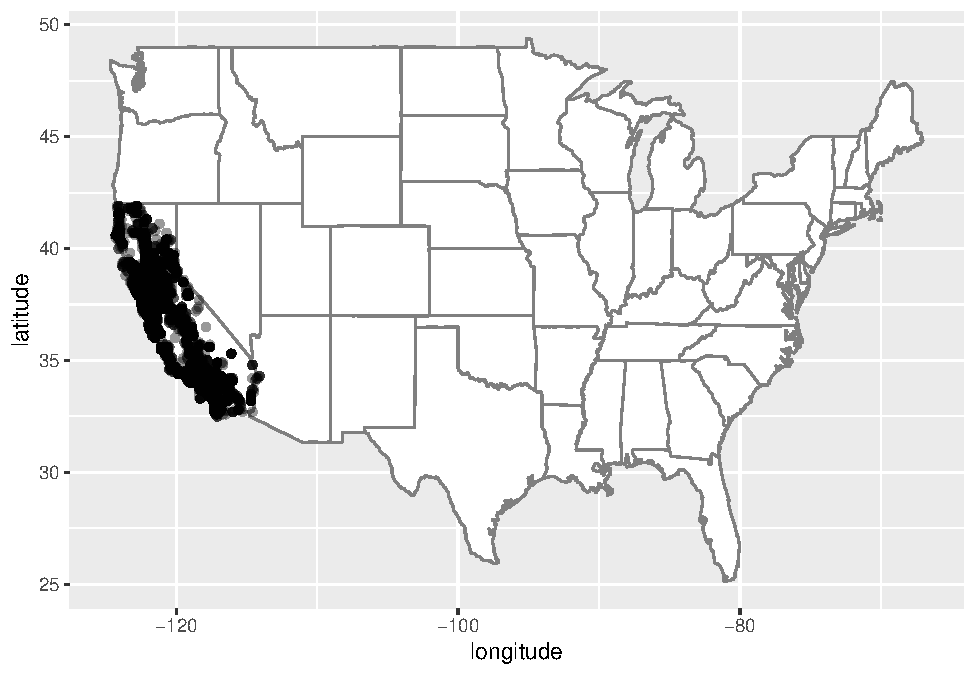
\includegraphics{ACT4114_TP_Part1_Equipe09_files/figure-latex/geolocalisation-1.pdf}

\begin{Shaded}
\begin{Highlighting}[]
\NormalTok{mapCalifornia }\OtherTok{\textless{}{-}} \FunctionTok{borders}\NormalTok{(}\AttributeTok{database =} \StringTok{"county"}\NormalTok{, }\AttributeTok{region =} \StringTok{"california"}\NormalTok{,}
                  \AttributeTok{colour=}\StringTok{"gray50"}\NormalTok{, }\AttributeTok{fill=}\StringTok{"white"}\NormalTok{)}
\FunctionTok{ggplot}\NormalTok{(}\AttributeTok{data =}\NormalTok{ data, }\FunctionTok{aes}\NormalTok{(}\AttributeTok{x =}\NormalTok{ longitude, }\AttributeTok{y =}\NormalTok{ latitude)) }\SpecialCharTok{+}
\NormalTok{    mapCalifornia }\SpecialCharTok{+} \FunctionTok{geom\_point}\NormalTok{(}\AttributeTok{alpha =}\NormalTok{ .}\DecValTok{4}\NormalTok{)}
\end{Highlighting}
\end{Shaded}

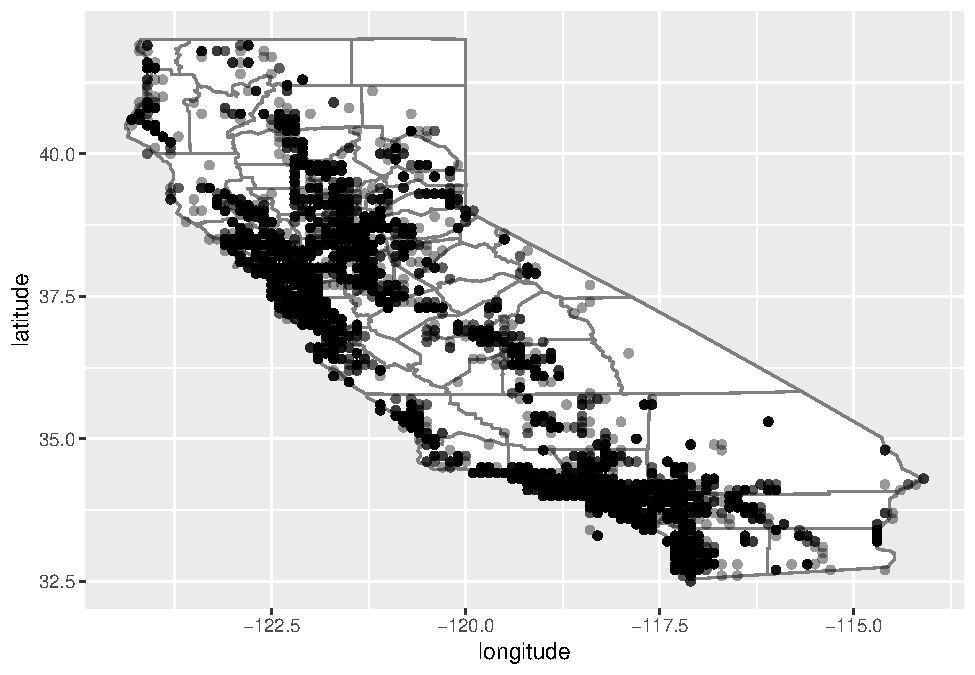
\includegraphics{ACT4114_TP_Part1_Equipe09_files/figure-latex/geolocalisation-2.pdf}

\begin{Shaded}
\begin{Highlighting}[]
\FunctionTok{md.pattern}\NormalTok{(data)}
\end{Highlighting}
\end{Shaded}

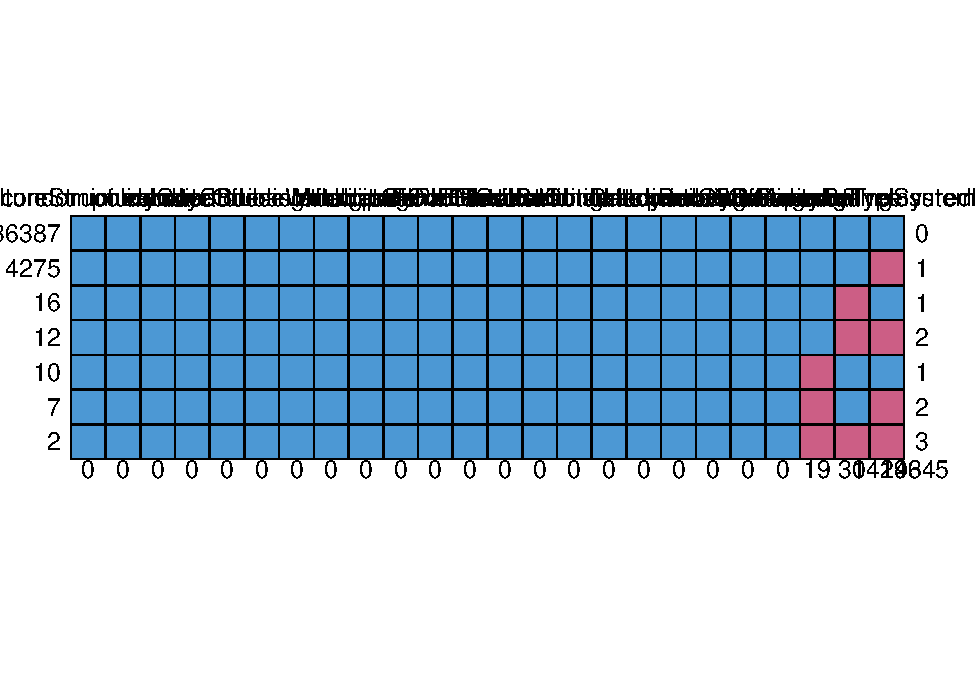
\includegraphics{ACT4114_TP_Part1_Equipe09_files/figure-latex/geolocalisation-3.pdf}

\begin{verbatim}
##       agricultureStructureIndicator condominiumIndicator policyCount countyCode
## 36387                             1                    1           1          1
## 14275                             1                    1           1          1
## 16                                1                    1           1          1
## 12                                1                    1           1          1
## 10                                1                    1           1          1
## 7                                 1                    1           1          1
## 2                                 1                    1           1          1
##                                   0                    0           0          0
##       dateOfLoss elevatedBuildingIndicator houseWorship latitude longitude
## 36387          1                         1            1        1         1
## 14275          1                         1            1        1         1
## 16             1                         1            1        1         1
## 12             1                         1            1        1         1
## 10             1                         1            1        1         1
## 7              1                         1            1        1         1
## 2              1                         1            1        1         1
##                0                         0            0        0         0
##       locationOfContents lowestFloorElevation nonProfitIndicator
## 36387                  1                    1                  1
## 14275                  1                    1                  1
## 16                     1                    1                  1
## 12                     1                    1                  1
## 10                     1                    1                  1
## 7                      1                    1                  1
## 2                      1                    1                  1
##                        0                    0                  0
##       originalConstructionDate postFIRMConstructionIndicator
## 36387                        1                             1
## 14275                        1                             1
## 16                           1                             1
## 12                           1                             1
## 10                           1                             1
## 7                            1                             1
## 2                            1                             1
##                              0                             0
##       smallBusinessIndicatorBuilding state totalBuildingInsuranceCoverage
## 36387                              1     1                              1
## 14275                              1     1                              1
## 16                                 1     1                              1
## 12                                 1     1                              1
## 10                                 1     1                              1
## 7                                  1     1                              1
## 2                                  1     1                              1
##                                    0     0                              0
##       totalContentsInsuranceCoverage yearOfLoss primaryResidence totalAmount
## 36387                              1          1                1           1
## 14275                              1          1                1           1
## 16                                 1          1                1           1
## 12                                 1          1                1           1
## 10                                 1          1                1           1
## 7                                  1          1                1           1
## 2                                  1          1                1           1
##                                    0          0                0           0
##       occupancyType numberOfFloorsInTheInsuredBuilding
## 36387             1                                  1
## 14275             1                                  1
## 16                1                                  0
## 12                1                                  0
## 10                0                                  1
## 7                 0                                  1
## 2                 0                                  0
##                  19                                 30
##       communityRatingSystemDiscount      
## 36387                             1     0
## 14275                             0     1
## 16                                1     1
## 12                                0     2
## 10                                1     1
## 7                                 0     2
## 2                                 0     3
##                               14296 14345
\end{verbatim}

\end{document}
